\title{Implementations}

\vspace{0.6 cm}

\noindent
This chapter presents the various implementations of the data validaion rules described in \ref{implementations}.

\section{VTL}

VTL

\section{Validate}

The \code{validate} package \citep{loo:2015} is build on top of the popular and
R language for statistical computing \citep{rcore:2015}. It is
implemented as an `R package' -- a strictly standardized way of distributing R
software, and publicly available through the Comprehensive R Archive Network
(CRAN). 

\subsubsection{The R language and environment}
The R language is an open source project, supported by the R foundation seated
in Vienna, Austria\footnote{\code{https://www.r-project.org/foundation/}}.
Over the last decade R received a surge in popularity both from research and
data science and business analytics communities. As a result R currently
integrates with every popular software system for data storage and processing,
including Microsoft SQL server, Oracle databases, Tibco Spotfire, Spark, and
Hadoop to name but a few.  Interaction with other programming environments such
as \code{C} and \code{C++}, \code{Java}, \code{.Net}, and \code{javascript} are
readily and freely available as well. The recently established R
consortium\footnote{\code{https://www.r-consortium.org/}} is an industry
initiative aimed to streamline and fund further developments in R.


The validate package is intended to be a small and powerful package that can be
used standalone by an analyst using R, or integrated easily into bigger
projects using one of the facilities mentioned above. As such, it is build with
strong adherence to the famous Unix
philosophy\footnote{\code{https://en.wikipedia.org/wiki/Unix\_philosophy}}: do
one thing, and do it really well.


\subsubsection{Approach for validate}
The philosophy behind the validate package is to reuse existing solutions as
much as possible. Most importantly, this means that rather than defining a
language from scratch, the validate package utilizes a subset of existing R
syntax for defining data validation rules. As an example, consider the following rule from the ESSnet survey \citep{walsdorfer:2015}.
\begin{quote}
Check whether the relative occurrence of the category high in a column
containing values low, high, medium does not exceed 10%.
\end{quote}
We assume a simple test dataset, with at least a column called \code{level}.
\begin{center}
\begin{tabular}{|c|}
\hline
\textbf{level}\\
\hline
medium\\
\hline
low\\
\hline
medium\\
\hline
medium\\
\hline
high\\
\hline
$\vdots$\\
\hline
\end{tabular}
\end{center}
In validate, the above rule translates to the following syntax.
\begin{verbatim}
  counts :=  table(level)
  counts["high"] < 0.1 * sum(counts)
\end{verbatim}
Here, \code{table} is a cross tabulation function that tabulates occurrences
of values in the \code{level} column. Since this function is a standard R
feature, tabulation or counting is not part of validate's syntax. Indeed the
validate package only makes sure that the statements issued by a user are in
fact validating statements as defined in the Hanbook on validation developed
for this project \citep{zio:2015}. In particular, this means that every
(statistical) transformation available to R can be part of a validating
statements.  With thousands of functions in base R, combined with the more than
7600 user-contributed packages available on CRAN, this results in a truly rich
set of validation functionality with a minimal cost of development and
maintenance to the authors.

Finally, we note that the approach of reusing R syntax for a specific purpose
is not new. Indeed several authors have created popular packages using the same
technology. Examples include an implementation of the famous grammar of
graphics \citep{wilkinson:2006} by \citet{wickham:2014}, the  `formula
interface' for statistical model specification and a grammar for data
manipulation by \cite{wickham:2014}. In fact, reusing existing languages, in
particular functional languages like R, is a well-established technique in
computer science.  Some key references for developing such embedded domain
specific languages (DSL) are \cite{fowler:2011} and \cite{gibbons:2015}.


\subsubsection{Features and usage}
Given that statistical functionality comes for free with R, the validate
package focuses only on features directly related to execution and maintenance
of validation rules and  analyses and presentation of validation results.
A few of the features are highlighted below.

\begin{description}
\item[Rule definition.] Rules can be defined on the R commandline for interactive
use or in text files that can be stored and manipulated as source code. Rule sets
may also be stored in a data base, since R by default supports connectivity to 
(nearly) any database that is (commercially) available.

\item[Rule metadata.] If so desired, rules can be provided with metadata such as
a time stamp, short and long descriptions, and the origin of the rule.  By
default, validate uses the widely supported YAML format for metadata
\citep{ben:2009}, mainly beacause of its human-readability. Since YAML can be
translated to formats like XML or JSON at the push of a button, communication
of rules between different softwares or machines is very easy.

\item[Rule organisation.] Dependencies between text files defining rules are
supported to allow for easy reuse of rules across different datasets.  A type
of \code{include} statement allows for hierarchical dependencies between rule
sets.

\item[Rule execution.] Validation rules can be confronted with any data that can
be read into R, which encompasses every common data format currently in use.
Of particular interest is \code{SDMX}, which is supported for R through a
package of \cite{bondel:2015}.

\item[Rule analyses.] Automatic detection of rule types, variable occurrence and
the rule dependency graph are currently built in. Add-on packages are currently
prototyped that will allow for detection of redundancies or contradictory rule
sets.

\item[Extensibility.] This is borrowed from R's extensibility. Users may define
functions which can be used in validating statements. The package needs no special
provisions for that.

\item[Integration.] Integration and communication with other is borrowed from
the strong features that R already has in this area. Because of its openness,
many interfaces with existing software and platforms, including commercial
ones, have been developed.

\item[Analyses of results.] The package has basic functionality to aggregate and
visualize results of validation  procedures. For example, one can sort records
according to the number of rule violations (record prioritization) or rules
according to which have been violated most often. Such summaries, and visualisations
thereof are important tools for monitoring data quality and the efficacy of 
data cleaning process steps \citep{pannekoek:2014}.
\end{description}

The \code{validate} package is the successor of an earlier package of the same
authors named \code{editrules}. The latter package has been used in production
for several years at Statistics Netherlands and is being evaluated by several
other national statistical institutes. At the moment, validate is being
introduced as editrules' replacement. The validate package is backwards
compatible with editrules in that it can read the same input files. However,
validate extends the earlier package by allowing for a much wider range of
validation rules (editrules was restricted to certain types of in-record
validation rules that are suitable for an error-localization algorithm).




\section{eSTATISTIK}

\subsubsection{The wider context}
The term \textit{eSTATISTIK} stands for a wider modernisation approach in German official statistics that has been ongoing for more than a decade and that aims at organising the transition from paper based to electronic production workflows and at the same time maximising its benefits in terms of efficiency, cost-effectiveness, flexibility, speed and quality. It involves all 15 German statistical institutes and therefore faces many issues that appear in a similar fashion at the European and international level. From a strategic perspective, standardisation in general and the movement from stove-pipe to cross-domain processes are important elements. This has led to the creation of generic applications and XML document types covering most steps of the production process. Specifically, the data collection process can be fully implemented using only generic metadata-driven applications, including data validation components for frontend and backend systems.

Another important strategic element is the consolidation and optimisation of the collaboration of the official statistical institutes and their partners. Its implementation requires adequate infrastructures for sharing and exchanging data and metadata throughout development and production life cycles, application hosting and sharing and the avoidance of duplicate work.

In the development and deployment phase, metadata are generated by tools used by domain experts for describing data sets, variables, validation rules and more. These metadata are deployed at specific metadata servers where they are accessible to internal production systems and partly to external users. This metadata infrastructure supports identifiers at the survey level, versioning and partitioning along observation areas (for accommodating resources specific to a single statistical institute). 

\subsubsection{Tools and infrastructure}


For data validation, a number of generic design and production tools exist. Figure~\ref{estattools} shows how those tools interact through the metadata infrastructure and the exchange of XML documents:

\begin{figure}[!ht]
\begin{center}
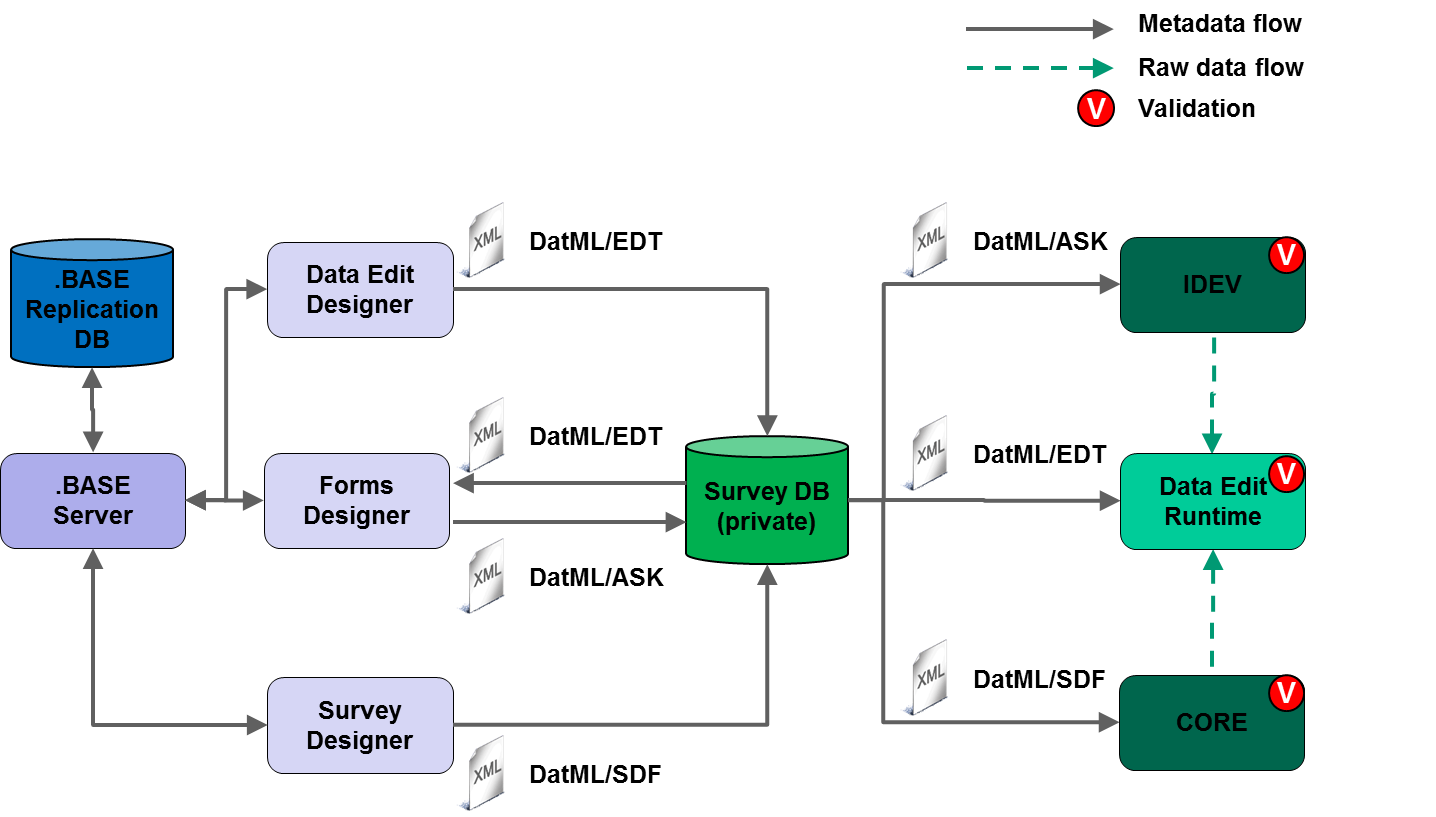
\includegraphics[scale=0.5]{fig/estattools.png} 
\end{center}
\caption{eSTATISTIK tools and their interaction}
\label{estattools}
\end{figure}

\begin{itemize}

\item
Domain experts use \textit{Data Edit Designer} for specifying data models for validation and editing (consisting of variables and variables groups, called \textit{topics}) and validation rules which are mainly used in web forms and back-end systems. Those specifications are exported in \textit{DatML/EDT} format. Validation rules can also be exported as Java classes.

\item
The \textit{Forms Designer} is used for designing web (and paper) forms. It resues data model and rule specifications made with the Data Edit Designer. Forms pecifications are exported in \textit{DatML/ASK} format.

\item
The \textit{Survey Designer} is used for specifying survey data models and front-end validation rules for the B2B data collection system \textit{CORE}.

\item
The \textit{Date Edit Runtime} is a generic platform for perfoming data validation. It is configured through DatML/EDT documents which are deployed along with data to be validated.

\end{itemize}

The design tools are part of the \textit{.BASE} tool suite. They are run as clients of a local .BASE server that provides central storage for metadata objects. A replication database is used for distributing metadata objects among statistical institutes. .BASE servers and the replication database provide the infrastructure for distributed development.

The \textit{Survey Database} serves metadata objects in XML format to production systems. A separate external instance of this database can be accessed by external users, specifically IT service and product providers and respondents.

Figure~\ref{estatinfra} shows the overall infrastructure for the data collection design and production processes:

\begin{figure}[!ht]
\begin{center}
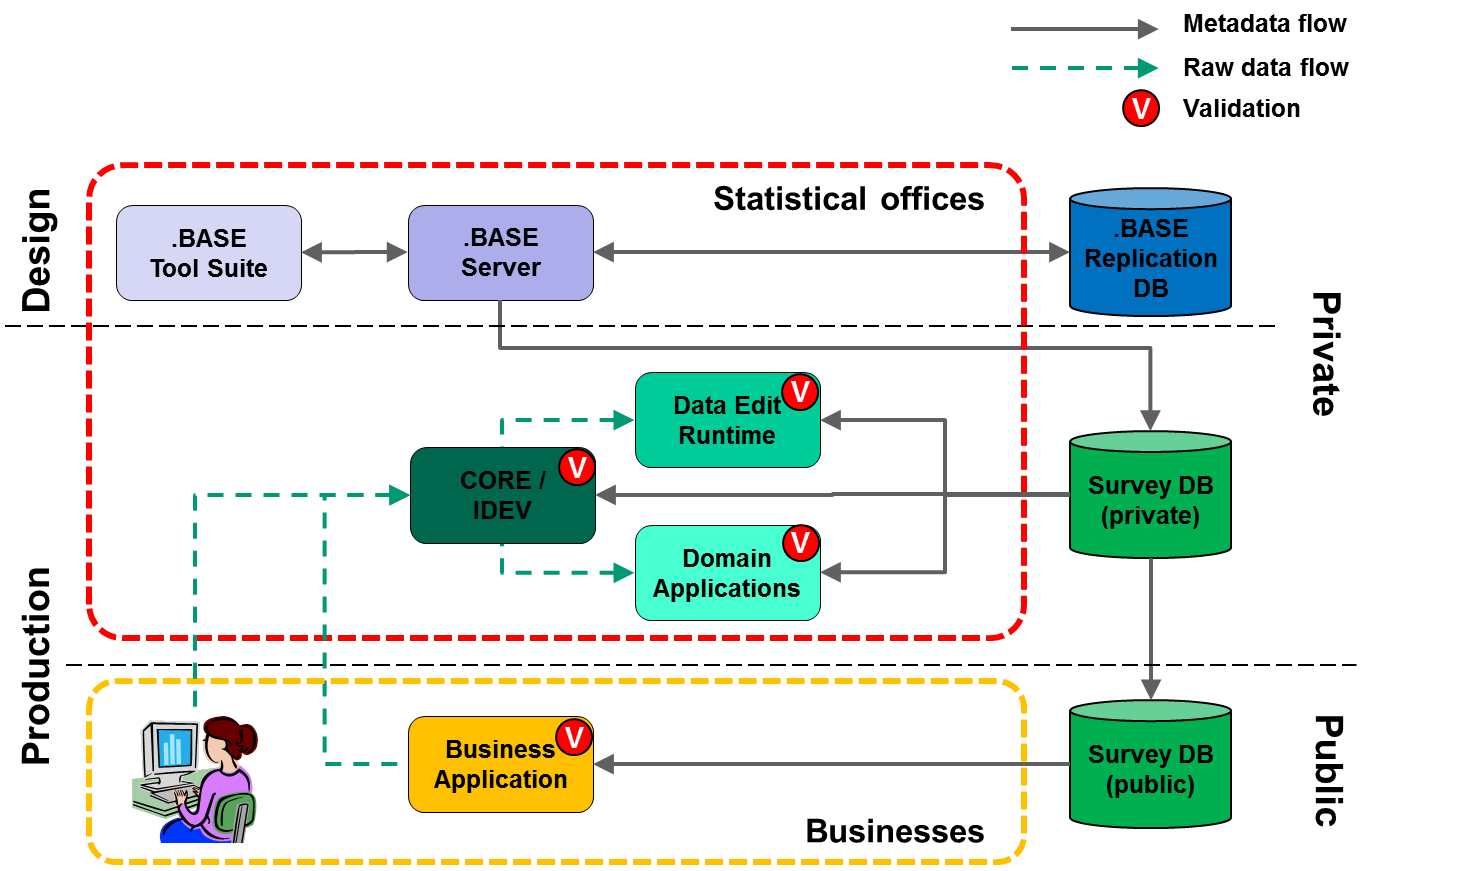
\includegraphics[scale=0.5]{fig/estatinfra.png} 
\end{center}
\caption{eSTATISTIK infrastructure for data collection design and production}
\label{estatinfra}
\end{figure}

\subsubsection{Specification language}

The eSTATISTIK specification language provides instructions for validating and editing data. There exist four programmatical contexts in which instructions can be used, and each context has its own restrictions as the the set of legal instructions. Awarenesss of those contexts is very important since they correspond to named programmatic objects that are edited and managed separately in the Date Edit Designer and Data Edit Runtime, but have some coding and runtime interdependencies. The four programmatical contexts are:

\begin{description}

\item[Procedures] serve to control the execution path of validation rules and automated edits, or in other words, to create and execute validation flows. Procedures can use the full instruction set of the specification language. Procedures can invoke other procedures conditionally as well as unconditionally, so that validation flows can be scoped and designed as building blocks, providing a means for modularisation and composition of data validation flows.

\item[Checks](a.k.a. validation rules) contain instructions for validating one or more columns/fields of the (hierarchical set of) record(s) currently in scope. Checks can only be invoked from procedures and have a very limited instruction set. They return TRUE if, and only if they encounter an error, otherwise FALSE. Only checks are evaluated for compiling validation statistics or metrics.

\item[Edits] are only invoked implicitly by checks that encounter an error (hard check). There is no instruction for invoking edits explicitly. An edit rule is therefore always bound to exactly one check and also has a very limited instruction set.

\item[Functions] provide a way for creating reusable units of code. Functions dispose of the full instructions set expect that checks cannot be invoked from functions. Functions can be invoked everywhere and recursively.

\end{description}

\subsubsection{Usage of tools}

In the execution environment Data Edit Runtime (DER), programmatic objects such as validation rules, reference data and other resources are bound to a survey node. Different versions of one resource can exist. A survey is associated with one or more reference periods. Reference periods serve to associate the data to be validated with (a version of) the resources used to perform the validation. For a given reference period, exactly one data set under validation can exist.

During execution of a validation flow, only the current record or the current set of hierarchical records (such as household and associated person records) of the data set under validation is visible and can be read and write accessed. Iterating over a complete data set is only possible in procedures and functions and if the data set is defined as reference data.

\subsubsection{Particularities of the PoC}

Files that serve as procedures have control in their file name, while all other .txt files represent simple validation rules.


The data used in the PoC provide some cases in which validation cannot be performed due to missing data. Those cases are recognisable by the value \code{undecided} in the column \code{expected} or in the data set name (where the full data set is validated), respectively. The idea behind this is to find out how systems differ in handling missing values. In eSTATISTIK, after executing a validation rule, the associated data are always considered validated, because validation rules only return TRUE or FALSE. Any precondition that may lead to a validation rule not being executed must be checked outside the rule, that is, in a procedure.
\code{Rule\_01} exemplifies this restriction. \code{Rule\_01.txt} contains the rule for validating the column  \code{hours\_worked} and is configured as a hard check (this configuration takes place in the rule editor). \code{Rule\_01.undecided.txt} only checks if \code{hours\_worked} is empty and represents a soft check. The procedure \code{Rule\_01\_control.txt} combines these checks, invoking \code{Rule\_01.txt} only if \code{Rule\_01.undecided.txt} returns FALSE, in which case \code{hours\_worked} is not empty. In this way, a soft error will be registered and displayed if the value is missing, and a hard error if a value is present but not within the valid range.



